\chapter{Edge Detection}

As mentioned earlier, road detection is performed in squares of 32 px. When determining the exact transition from road to non-road, the best possible accuracy is 32 px. 
\npar --- nog verder aanvullen: edge detectie voor hogere nauwkeurigheid van de exacte overgang van weg naar niet-weg en voor fallback op wegdetectie bij slechte wegen, zoals kasseiwegen 

\subsection{Removing details}

Detecting edges is very straightforward using an edge detection algorithm like Canny Edge Detection. However, there are a lot of edges on the road itself, thinking of road markings and cobbles. The edges on the road, considerd as noise, and the edges of the road are not unambiguously separable. The width of the patterns that cause the edges on the road is rather small. Using morphological image processing operations, it is possible to remove these small patterns from the image.  
\npar
Eroding is

Kasseien: kassei zelf is het helderste (voorgrond),  krimpt --> voeg groeit, tot het één oppervlak vormt
Lijnen: Lijn is het helderste (voorgrond), krimpt --> verdwijnt

Nadien: alle donkere objecten groter geworden, compenseren via dilatie

\begin{figure}[ht]
\centering
\begin{subfigure}{.5\textwidth}
  \centering
  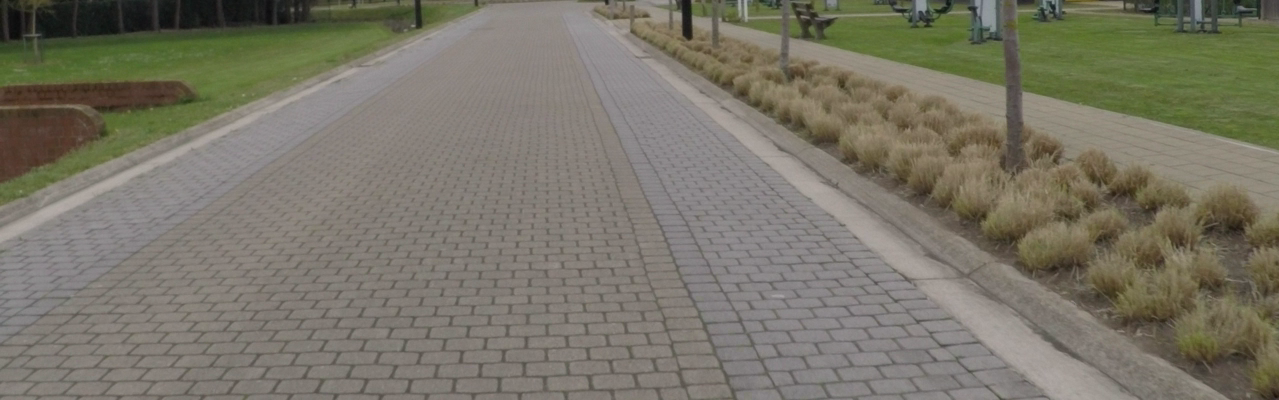
\includegraphics[width=.9\textwidth]{cobbles_in}
  \caption{Original frame\label{zebra_orig}}
\end{subfigure}%
\begin{subfigure}{.5\textwidth}
  \centering
  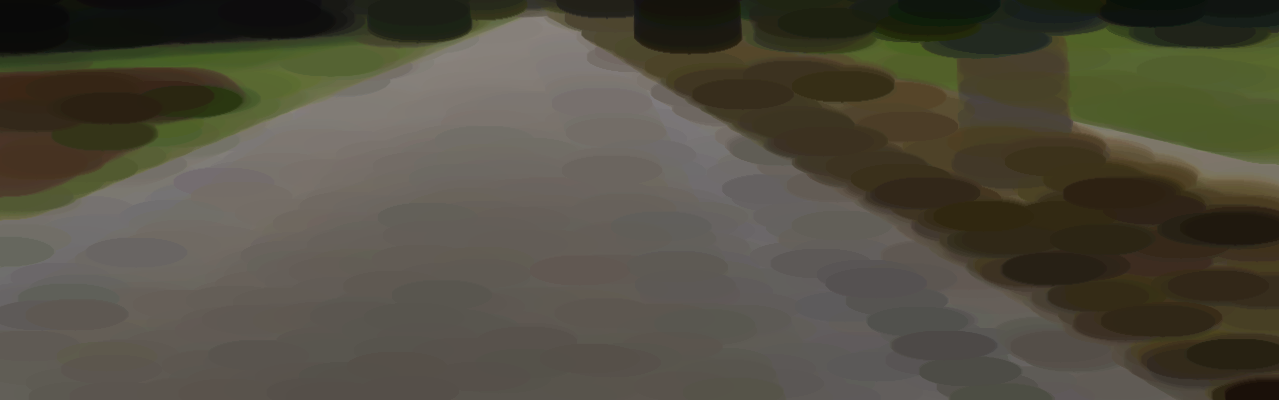
\includegraphics[width=.9\textwidth]{cobbles_erode_out}
  \caption{Objects become bigger after eroding\label{zebrawitcanny}}
\end{subfigure}
\caption{Perform eroding and dilation to remove details.}
\end{figure}


\begin{figure}[ht]
\centering
\begin{subfigure}{.5\textwidth}
  \centering
  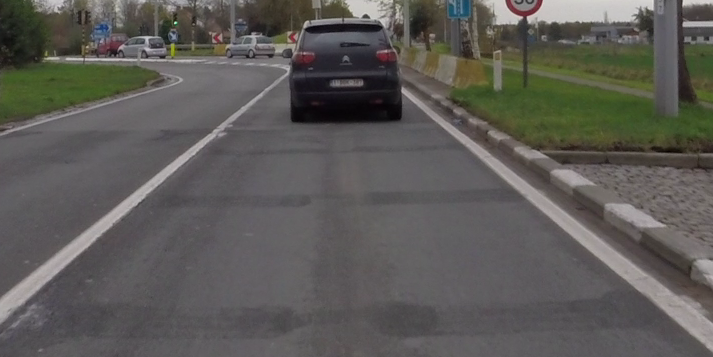
\includegraphics[width=.9\textwidth]{car_original}
  \caption{Original frame\label{zebra_orig}}
\end{subfigure}%
\begin{subfigure}{.5\textwidth}
  \centering
  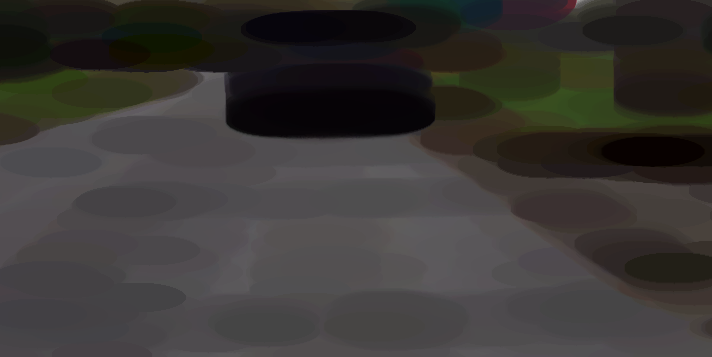
\includegraphics[width=.9\textwidth]{car_erode_bigger}
  \caption{Objects become bigger after eroding\label{zebrawitcanny}}
\end{subfigure}
\begin{subfigure}{.5\textwidth}
  \centering
  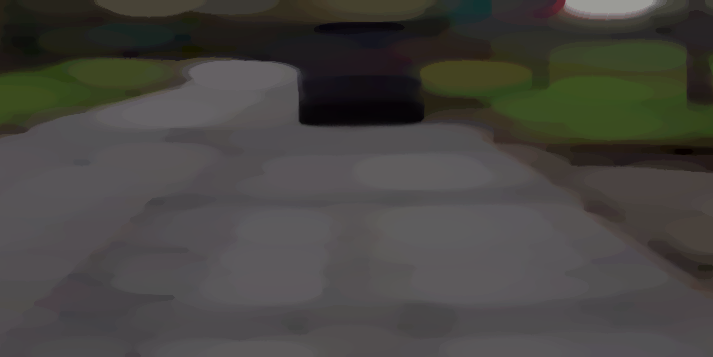
\includegraphics[width=.9\textwidth]{car_dilate_smaller}
  \caption{Restore original sizes with dilation\label{zebrawitcanny}}
\end{subfigure}
\caption{Perform eroding and dilation to remove details.}
\end{figure}


\subsection{Canny Edge Detection}